
\section{MTL4}

\begin{frame}[fragile]

 \heading{Calculate an ensemble of pendulums}

 \begin{lstlisting}[basicstyle=\scriptsize\ttfamily]
typedef mtl::dense_vector<double> vector_type;
typedef mtl::multi_vector<vector_type> state_type;
typedef runge_kutta4<state_type,double,state_type,double,
  vector_space_algebra,default_operations> stepper_type;

state_type X(N, 2);
vector_type Eps(N), Omega(N);

// initialize x, Eps, Omega
integrate_const(stepper(), ensemble(Eps, Omega, 0.1) ,
    X, 0.0, t_max, dt);
 \end{lstlisting}

\vspace{2ex}

\centerline{Memory layout:}

\vspace{1ex}

\centerline{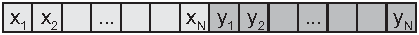
\includegraphics[draft=false,width=0.7\textwidth]{memory_layout2.pdf}}

\vspace{2ex}

\centerline{Everything seems easy!}
\vspace{2ex}
\centerline{{\bf But} how does {\tt ensemble} look like?}
 

\end{frame}




\begin{frame}[fragile]

 \heading{Ensemble of nonlinear pendulums}

 \begin{lstlisting}[basicstyle=\scriptsize\ttfamily]
struct ensemble
{
  const vector_type &m_eps, &m_omega;
  double m_mu;

  ensemble(const vector_type &eps,const vector_type &omega,
    double mu)
      : m_eps(eps), m_omega(omega), m_mu(mu) { }

  void operator()(const state_type &x, state_type &dxdt,
    double t)
  {
    dxdt.at(0)= x.at(1);
    dxdt.at(1)= -sin(x.at(0)) - m_mu*x.at(1) + m_eps*sin(m_omega*t);
  }
};
 \end{lstlisting}

\end{frame}

\begin{frame}
  \heading{What is MTL4?}
  \begin{itemize}
  \item Matrix Template Library v4
  \item A Library for linear algebra
  \item It provides an intuitive interface
  \item Similar to Matlab
    \begin{itemize}
    \item Translators Matlab $\rightarrow$ MTL4 in progress
    \end{itemize}
  \item Simplicity without sacrificing performance
  \item Portability with little or no code change

  \end{itemize}

\end{frame}

\begin{frame}
  \heading{DSEL for intuitive use}
  \begin{itemize}
  \item The number of operations is limited.
  \item But the number of types is not.
  \end{itemize}
  \small
  \begin{tabbing}
  \= A[iset\{2, 4, 3\}][iset\{8, 1\}] bla\= \code{A[irange][irange]} bla \=general sub-matrix; bla\= df \kill
  \>A[3][7]\> \code{A[int][int]}\> matrix element\\
  \>A[iall][irange(3, 7)]\> \code{A[irange][irange]}\> sub-matrix\\
  \>A[4][irange(2, imax)]\> \code{A[int][irange]}\> row vector\\
  \>A[iall][3]\> \code{A[irange][int]}\> column vector\\
  \>A[iset\{2, 4, 3\}][iset\{8, 1\}]\> \code{A[iset][iset]}\> general sub-matrix \\
\end{tabbing}
\end{frame}


\begin{frame}[containsverbatim]
\heading{Example application: LU}
\begin{lstlisting}
template <typename Matrix>
void inline lu(Matrix& LU)
{
    MTL_THROW_IF(num_rows(LU) != num_cols(LU), matrix_not_square());

    for (std::size_t k= 0; k < num_rows(LU)-1; k++) {
	irange r(k+1, imax); // Interval [k+1, n-1]
	LU[r][k]/= LU[k][k];
	LU[r][r]-= LU[r][k] * LU[k][r];
    }
}
\end{lstlisting}
\end{frame}



%\subsection{Our Vision of Portable Programming}

\swvision{Folie1}
\swvision{Folie2}
\swvision{Folie3}
\swvision{Folie4}
\swvision{Folie5}
\swvision{Folie6}
\swvision{Folie7}
\swvision{Folie8}
\swvision{Folie9}
\swvision{Folie10}
\swvision{Folie11}
\addtocounter{framenumber}{1}




\begin{frame}
  \heading{Challenges with CUDA}
  \begin{itemize}
  \item No support for complex,
  \item No mixed arithmetic,
  \item Intrinsically only flat copies,
    \begin{itemize}
    \item Limits applicability of user types,
    \end{itemize}
  \item Many algorithms difficult or impossible on GPU
  \end{itemize}

\end{frame}

\begin{frame}
  \heading{Dynamic Memory Management}
  \begin{itemize}
  \item Dynamic memory management and heterogeneity
  \item Complex data structures easier to initialize on CPU
  \item Likewise for I/O
    \begin{itemize}
    \item Reuse of CPU implementation
    \end{itemize}
  \item Small data can be handled on CPU
  \item Types with and w/o CUDA support can be mixed
  \end{itemize}
\end{frame}


\begin{frame}
  \heading{Debugging}
  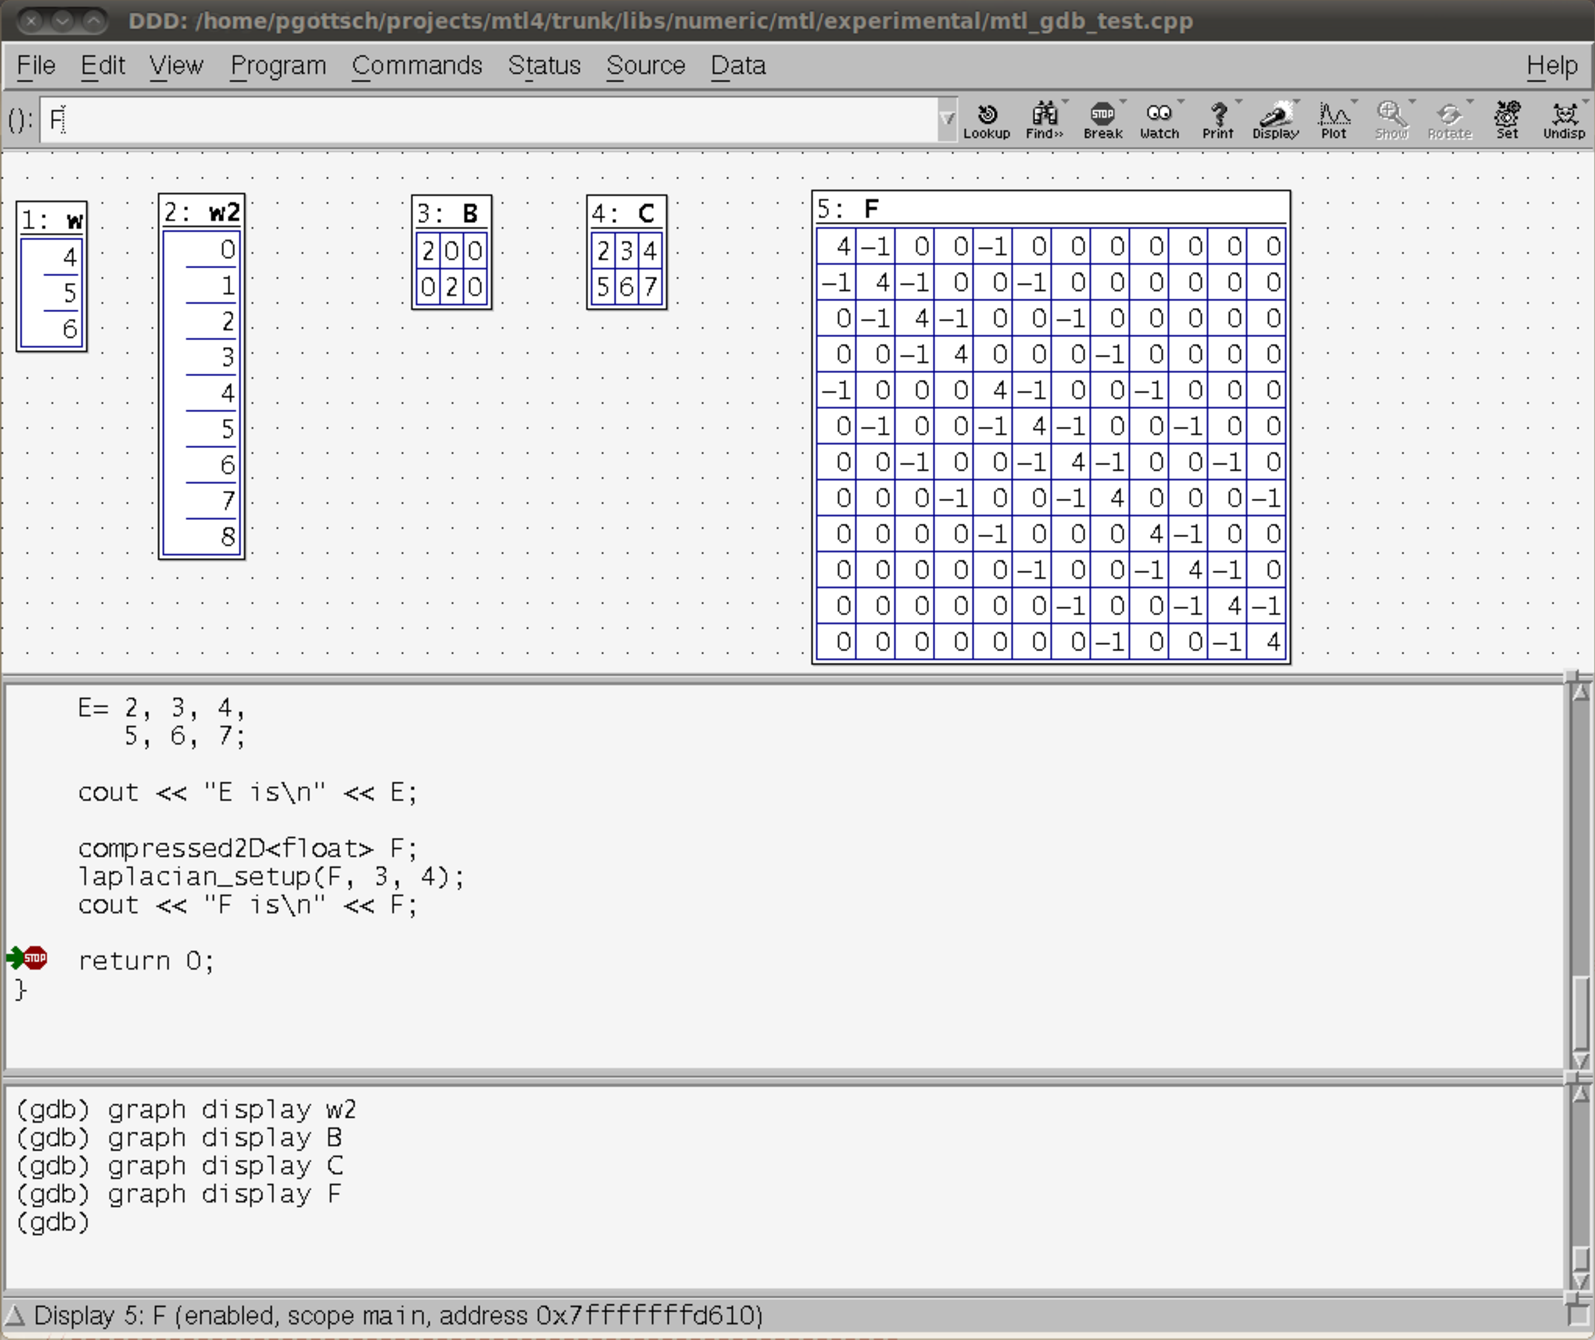
\includegraphics[width=0.82\columnwidth]{DDD.pdf}
\end{frame}


% \begin{frame}
%   \heading{Portability}
%   \begin{itemize}
%   \item Same abstractions and interfaces for
%     \begin{itemize}
%     \item Sequential MTL4,
%     \item CUDA-MTL4, and
%     \item Parallel MTL4.
%     \end{itemize}
%   \item Entirely generic design
%     \begin{itemize}
%     \item In fact, most of the code is identic
%     \end{itemize}
%   \end{itemize}
% \end{frame}
